% THIS IS AN EXAMPLE DOCUMENT FOR VLDB 2012
% based on ACM SIGPROC-SP.TEX VERSION 2.7
% Modified by  Gerald Weber <gerald@cs.auckland.ac.nz>
% Removed the requirement to include *bbl file in here. (AhmetSacan, Sep2012)
% Fixed the equation on page 3 to prevent line overflow. (AhmetSacan, Sep2012)

\documentclass{vldb}
\usepackage{graphicx}
\usepackage{balance}  % for  \balance command ON LAST PAGE  (only there!)
\usepackage{fontspec}
\usepackage{hyperref}
\graphicspath{{figures/}}
\usepackage{enumitem}

\begin{document}

% ****************** TITLE ****************************************

\title{Druid: Open Source Real-time Analytics at Scale}

% possible, but not really needed or used for PVLDB:
%\subtitle{[Extended Abstract]
%\titlenote{A full version of this paper is available as\textit{Author's Guide to Preparing ACM SIG Proceedings Using \LaTeX$2_\epsilon$\ and BibTeX} at \texttt{www.acm.org/eaddress.htm}}}

% ****************** AUTHORS **************************************

% You need the command \numberofauthors to handle the 'placement
% and alignment' of the authors beneath the title.
%
% For aesthetic reasons, we recommend 'three authors at a time'
% i.e. three 'name/affiliation blocks' be placed beneath the title.
%
% NOTE: You are NOT restricted in how many 'rows' of
% "name/affiliations" may appear. We just ask that you restrict
% the number of 'columns' to three.
%
% Because of the available 'opening page real-estate'
% we ask you to refrain from putting more than six authors
% (two rows with three columns) beneath the article title.
% More than six makes the first-page appear very cluttered indeed.
%
% Use the \alignauthor commands to handle the names
% and affiliations for an 'aesthetic maximum' of six authors.
% Add names, affiliations, addresses for
% the seventh etc. author(s) as the argument for the
% \additionalauthors command.
% These 'additional authors' will be output/set for you
% without further effort on your part as the last section in
% the body of your article BEFORE References or any Appendices.

\numberofauthors{6} %  in this sample file, there are a *total*
% of EIGHT authors. SIX appear on the 'first-page' (for formatting
% reasons) and the remaining two appear in the \additionalauthors section.

\author{
% You can go ahead and credit any number of authors here,
% e.g. one 'row of three' or two rows (consisting of one row of three
% and a second row of one, two or three).
%
% The command \alignauthor (no curly braces needed) should
% precede each author name, affiliation/snail-mail address and
% e-mail address. Additionally, tag each line of
% affiliation/address with \affaddr, and tag the
% e-mail address with \email.
%
% 1st. author
\alignauthor
Fangjin Yang\\
       \affaddr{Metamarkets Group, Inc.}\\
       \email{fangjin@metamarkets.com}
% 2nd. author
\alignauthor
Eric Tschetter\\
       \email{echeddar@gmail.com}
% 3rd. author
\alignauthor 
Xavier Léauté\\
       \affaddr{Metamarkets Group, Inc.}\\
       \email{xavier@metamarkets.com}
\and  % use '\and' if you need 'another row' of author names
% 4th. author
\alignauthor
Nishant Bangarwa\\
       \affaddr{Metamarkets Group, Inc.}\\
       \email{nishant@metamarkets.com}
% 5th. author
\alignauthor
Nelson Ray\\
       \email{ncray86@gmail.com}
% 6th. author
\alignauthor
Gian Merlino\\
       \affaddr{Metamarkets Group, Inc.}\\
       \email{gian@metamarkets.com}
}
% There's nothing stopping you putting the seventh, eighth, etc.
% author on the opening page (as the 'third row') but we ask,
% for aesthetic reasons that you place these 'additional authors'
% in the \additional authors block, viz.
\additionalauthors{Additional authors: Deep Ganguli (Metamarkets Group, Inc., {\texttt{deep@metamarkets.com}}), Himadri Singh (Metamarkets Group, Inc., {\texttt{himadri@metamarkets.com}}), Igal Levy (Metamarkets Group, Inc., {\texttt{igal@metamarkets.com}})}
\date{14 March 2014}
% Just remember to make sure that the TOTAL number of authors
% is the number that will appear on the first page PLUS the
% number that will appear in the \additionalauthors section.


\maketitle

\begin{abstract}
Druid is an open
source\footnote{\href{https://github.com/apache/druid}{https://github.com/apache/druid}}
data store built for exploratory analytics on large data sets.  Druid supports
fast data aggregation, low latency data ingestion, and arbitrary data
exploration. The system combines a column-oriented storage layout, a
distributed, shared-nothing architecture, and an advanced indexing structure to
return queries on billions of rows in milliseconds.  Druid is petabyte scale and
is deployed in production at several technology companies.
\end{abstract}

\section{Introduction}
The recent proliferation of internet technology has created a surge
in machine-generated events.  Individually, these events contain minimal useful
information and are of low value.  Given the time and resources required to
extract meaning from large collections of events, many companies were willing
to discard this data instead.  

A few years ago, Google introduced MapReduce as their mechanism of leveraging
commodity hardware to index the internet and analyze logs.  The Hadoop project
soon followed and was largely patterned after the insights that came out of the
original MapReduce paper. Hadoop has contributed much to helping companies
convert their low-value event streams into high-value aggregates for a variety
of applications such as business intelligence and A-B testing.

As with a lot of great systems, Hadoop has opened our eyes to a new space of
problems.  Specifically, Hadoop excels at storing and providing access to large
amounts of data, however, it does not make any performance guarantees around
how quickly that data can be accessed.  Furthermore, although Hadoop is a
highly available system, performance degrades under heavy concurrent load.
Lastly, while Hadoop works well for storing data, it is not optimized for
ingesting data and making that data immediately readable.

\subsection{The Need for Druid}
Druid was originally designed to solve problems around ingesting and exploring
large quantities of transactional events (log data). This form of timeseries
data (OLAP data) is commonly found in the business intelligence
space and the nature of the data tends to be very append heavy. Events typically
have three distinct components: a timestamp column indicating when the event
occurred, a set of dimension columns indicating various attributes about the
event, and a set of metric columns containing values (usually numeric) that can
be aggregated. Queries are typically issued for the sum of some set of metrics,
filtered by some set of dimensions, over some span of time. 

The Druid project first began out of necessity at Metamarkets to power a
business intelligence dashboard that allowed users to arbitrarily explore and
visualize event streams. Existing open source Relational Database Management
Systems, cluster computing frameworks, and NoSQL key/value stores were unable
to provide a low latency data ingestion and query platform for an interactive
dashboard. Queries needed to return fast enough to allow the data
visualizations in the dashboard to update interactively.

In addition to the query latency needs, the system had to be multi-tenant and
highly available, as the dashboard is used in a highly concurrent environment.
Downtime is costly and many businesses cannot afford to wait if a system is
unavailable in the face of software upgrades or network failure. Finally,
Metamarkets also wanted to allow users and alerting systems to be able to make
business decisions in ``real-time". The time from when an event is created to
when that event is queryable determines how fast users and systems are able to
react to potentially catastrophic occurrences in their systems. 

The problems of data exploration, ingestion, and availability span multiple
industries. Since Druid was open sourced in October 2012, it has been deployed as a
video, network monitoring, operations monitoring, and online advertising
analytics platform at multiple companies\footnote{\href{http://druid.org/apache/druid.html}{http://druid.org/apache/druid.html}}.

\begin{figure*}
\centering
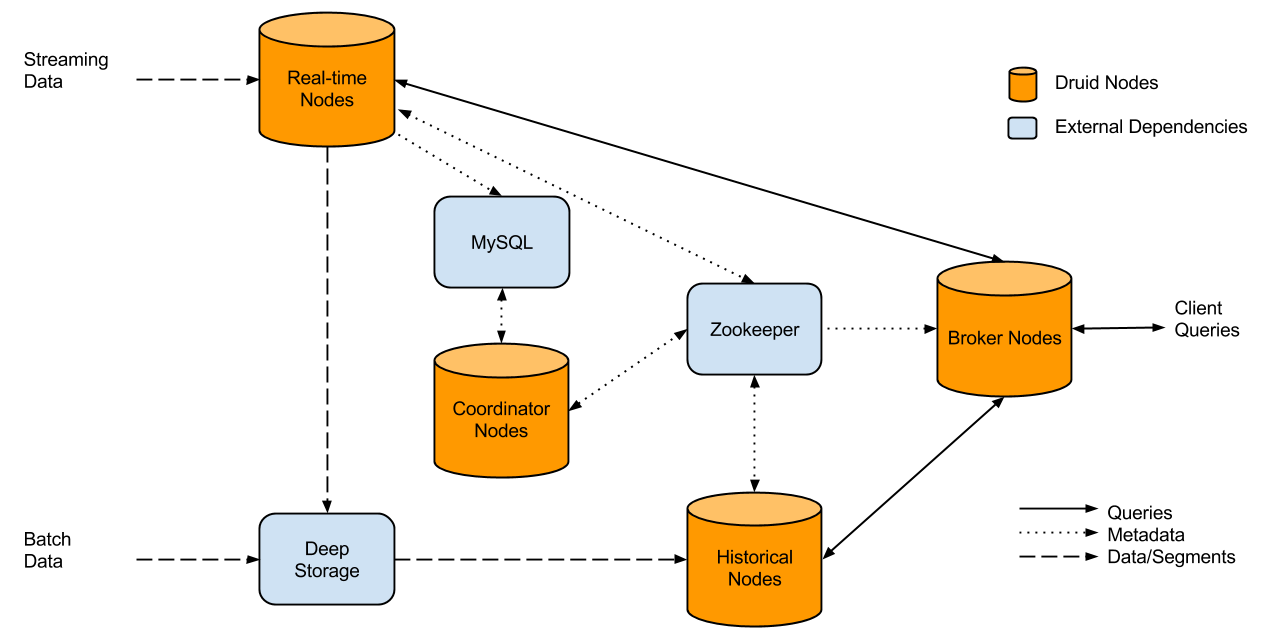
\includegraphics[width = 4.5in]{cluster}
\caption{An overview of a Druid cluster and the flow of data through the cluster.}
\label{fig:cluster}
\end{figure*}

\section{Architecture}
A Druid cluster consists of different types of nodes and each node type is
designed to perform a specific set of things. We believe this design separates
concerns and simplifies the complexity of the system. The different node types
operate fairly independently of each other and there is minimal interaction among
them. Hence, intra-cluster communication failures have minimal impact on data
availability.  To solve complex data analysis problems, the different node
types come together to form a fully working system. The composition of and flow
of data in a Druid cluster are shown in Figure~\ref{fig:cluster}. All Druid
nodes announce their availability and the data they are serving over
Zookeeper\cite{hunt2010zookeeper}.

\subsection{Real-time Nodes}
Real-time nodes encapsulate the functionality to ingest and query event
streams. Events indexed via these nodes are immediately available for querying.
These nodes are only concerned with events for some small time range. They
periodically hand off batches of immutable events to other nodes in the Druid
cluster that are specialized in dealing with batches of immutable events.

Real-time nodes maintain an in-memory index buffer for all incoming events.
These indexes are incrementally populated as new events are ingested and the
indexes are also directly queryable. To avoid heap overflow problems, real-time
nodes persist their in-memory indexes to disk either periodically or after some
maximum row limit is reached. This persist process converts data stored in the
in-memory buffer to a column oriented storage format. Each persisted index is
immutable and real-time nodes load persisted indexes into off-heap memory such
that they can still be queried. On a periodic basis, each real-time node will
schedule a background task that searches for all locally persisted indexes. The
task merges these indexes together and builds an immutable block of data that
contains all the events that have ingested by a real-time node for some span of
time. We refer to this block of data as a ``segment". During the handoff stage,
a real-time node uploads this segment to permanent backup storage, typically
a distributed file system that Druid calls ``deep storage".

\subsection{Historical Nodes}
Historical nodes encapsulate the functionality to load and serve the immutable
blocks of data (segments) created by real-time nodes. In many real-world
workflows, most of the data loaded in a Druid cluster is immutable and hence
historical nodes are typically the main workers of a Druid cluster.  Historical
nodes follow a shared-nothing architecture and there is no single point of
contention among the nodes. The nodes have no knowledge of one another and are
operationally simple; they only know how to load, drop, and serve immutable
segments.

\subsection{Broker Nodes}
Broker nodes act as query routers to historical and real-time nodes. Broker
nodes understand what segments are queryable and where those segments are
located. Broker nodes route incoming queries such that the queries hit the
right historical or real-time nodes. Broker nodes also merge partial results
from historical and real-time nodes before returning a final consolidated
result to the caller.

\subsection{Coordinator Nodes}
Druid coordinator nodes are primarily in charge of data management and
distribution on historical nodes. The coordinator nodes tell historical nodes
to load new data, drop outdated data, replicate data, and move data to load
balance. Coordinator nodes undergo a
leader-election process that determines a single node that runs the coordinator
functionality. The remaining coordinator nodes act as redundant backups.

A coordinator node runs periodically to determine the current state of the
cluster. It makes decisions by comparing the expected state of the cluster with
the actual state of the cluster at the time of the run.  Coordinator nodes also
maintain a connection to a MySQL database that contains additional operational
parameters and configurations.  One of the key pieces of information located in
the MySQL database is a table that contains a list of all segments that should
be served by historical nodes.  This table can be updated by any service that
creates segments, such as real-time nodes. 

\subsection{Query Processing}
Data tables in Druid (called \emph{data sources}) are collections of
timestamped events partitioned into a set of segments, where each segment
is typically 5--10 million rows. Formally, we define a segment as a collection
of rows of data that span some period in time. Segments represent the
fundamental storage unit in Druid and replication and distribution are done at
a segment level.

Druid segments are stored in a column orientation. Given that Druid is best
used for aggregating event streams (all data going into Druid must have a
timestamp), the advantages storing aggregate information as columns rather than
rows are well documented \cite{abadi2008column}. Column storage allows for more
efficient CPU usage as only what is needed is actually loaded and scanned. 

Druid has multiple column types to represent various data formats. Depending on
the column type, different compression methods are used to reduce the cost of
storing a column in memory and on disk. For example, if an entire column only
contains string values, storing the raw strings is unnecessarily costly.
String columns can be dictionary encoded instead. Dictionary encoding is a
common method to compress data in column stores.

In many real world OLAP workflows, queries are issued for the aggregated
results of some set of metrics where some set of dimension specifications are
met. Consider Table~\ref{tab:sample_data}. An example query for this table may
ask: ``How much revenue was generated in the first hour of 2014-01-01 in the
city of San Francisco?". This query is filtering a sales data set based on a
Boolean expression of dimension values. In many real world data sets, dimension
columns contain strings and metric columns contain numbers. Druid creates
additional lookup indices for string columns such that only those rows that
pertain to a particular query filter are ever scanned.

\begin{table}
  \centering
  \begin{tabular}{| l | l | l |}
    \hline
    \textbf{Timestamp} & \textbf{City} & \textbf{Revenue} \\ \hline
    2014-01-01T01:00:00Z & San Francisco & 25 \\ \hline
    2014-01-01T01:00:00Z & San Francisco & 42 \\ \hline
    2014-01-01T02:00:00Z & New York & 17 \\ \hline
    2014-01-01T02:00:00Z & New York & 170 \\ \hline
  \end{tabular}
  \caption{Sample sales data set.}
  \label{tab:sample_data}
\end{table}

For each unique city in
Table~\ref{tab:sample_data}, we can form some representation
indicating in which table rows a particular city is seen. We can
store this information in a binary array where the array indices
represent our rows. If a particular page is seen in a certain
row, that array index is marked as \texttt{1}. For example:
{\small\begin{verbatim}
San Francisco -> rows [0, 1] -> [1][1][0][0]
New York      -> rows [2, 3] -> [0][0][1][1]
\end{verbatim}}

\texttt{San Francisco} is seen in rows \texttt{0} and \texttt{1}. This mapping of column values
to row indices forms an inverted index \cite{tomasic1993performance}. To know which
rows contain {\ttfamily San Francisco} or {\ttfamily New York}, we can \texttt{OR} together
the two arrays.
{\small\begin{verbatim}
[0][1][0][1] OR [1][0][1][0] = [1][1][1][1]
\end{verbatim}}

This approach of performing Boolean operations on large bitmap sets is commonly
used in search engines. Druid compresses each bitmap index using the Concise
algorithm \cite{colantonio2010concise}. All Boolean operations on top of these
Concise sets are done without decompressing the set. 

\subsection{Query Capabilities}
Druid supports many types of aggregations including double sums, long sums,
minimums, maximums, and complex aggregations such as cardinality estimation and
approximate quantile estimation.  The results of aggregations can be combined
in mathematical expressions to form other aggregations. Druid supports
different query types ranging from simple aggregates for an interval time,
groupBys, and approximate top-K queries. 

\section{Performance}
Druid runs in production at several organizations, and to briefly demonstrate its
performance, we have chosen to share some real world numbers for the main production
cluster running at Metamarkets in early 2014. For comparison with other databases
we also include results from synthetic workloads on TPC-H data.

\subsection{Query Performance}
Query latencies are shown in Figure~\ref{fig:query_latency} for a cluster
hosting approximately 10.5TB of data using 1302 processing threads and 672
total cores (hyperthreaded). There are approximately 50 billion rows of data in
this cluster.

\begin{figure}
\centering
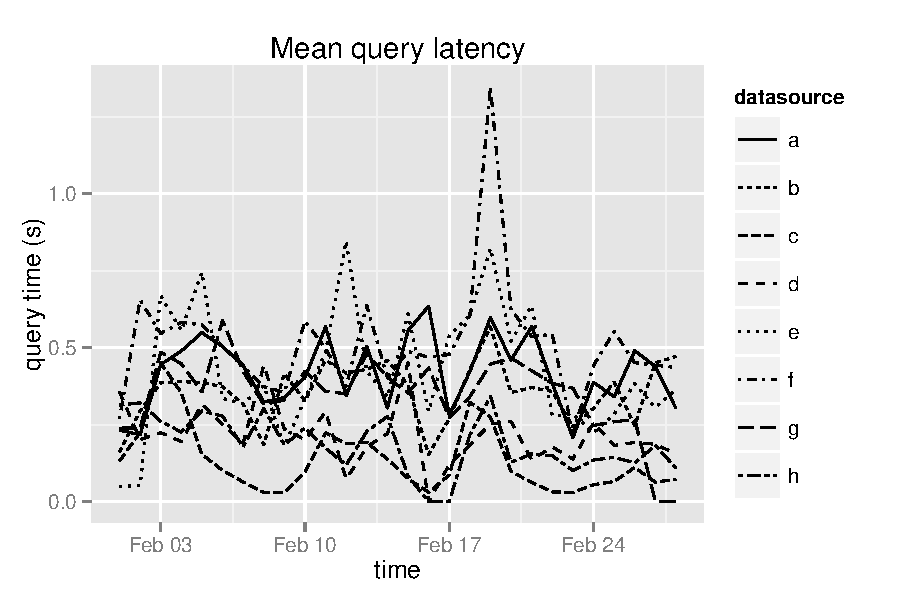
\includegraphics[width = 2.3in]{avg_query_latency}
\caption{Query latencies of production data sources.}
\label{fig:query_latency}
\end{figure}

\begin{figure}
\centering
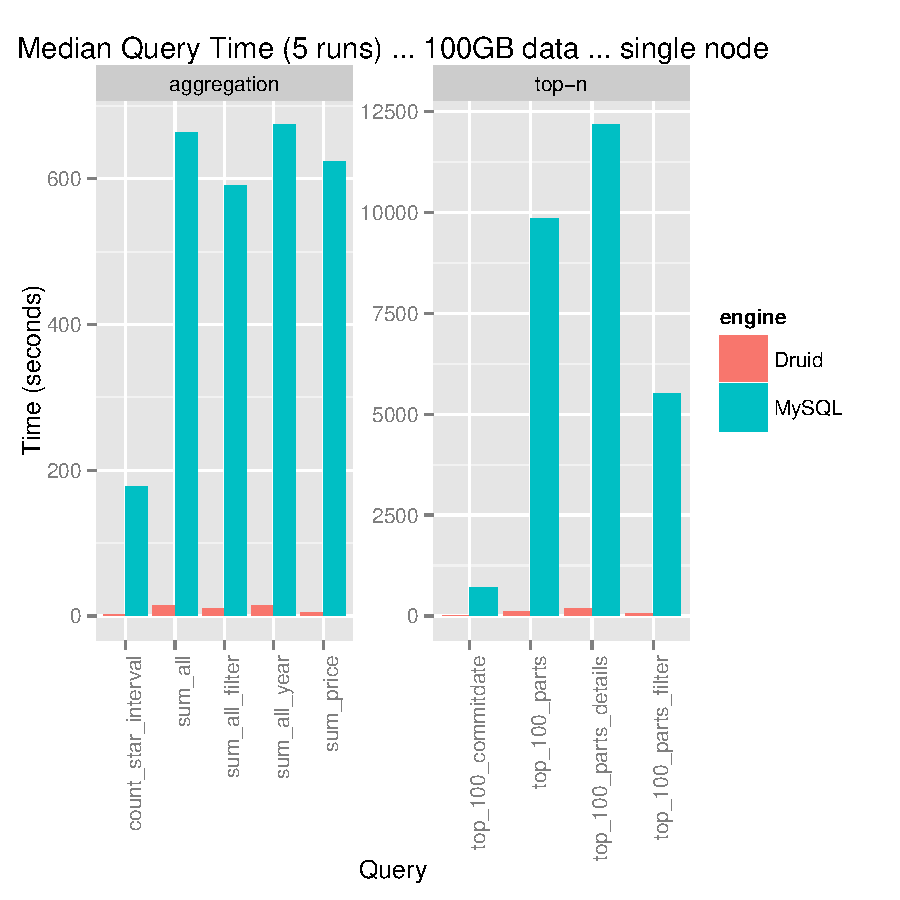
\includegraphics[width = 2.3in]{tpch_100gb}
\caption{Druid \& MySQL benchmarks -- 100GB TPC-H data.}
\label{fig:tpch_100gb}
\end{figure}

The average queries per minute during this time was approximately
1000. The number of dimensions the various data sources vary from 25 to 78
dimensions, and 8 to 35 metrics. Across all the various data sources, average
query latency is approximately 550 milliseconds, with 90\% of queries returning
in less than 1 second, 95\% in under 2 seconds, and 99\% of queries returning
in less than 10 seconds.  

Approximately 30\% of the queries are standard
aggregates involving different types of metrics and filters, 60\% of queries
are ordered group bys over one or more dimensions with aggregates, and 10\% of
queries are search queries and metadata retrieval queries. The number of
columns scanned in aggregate queries roughly follows an exponential
distribution. Queries involving a single column are very frequent, and queries
involving all columns are very rare.

We also present Druid benchmarks on TPC-H data in Figure~\ref{fig:tpch_100g}.
Most TPC-H queries do not directly apply to Druid, so we selected queries more
typical of Druid's workload to demonstrate query performance. As a comparison,
we also provide the results of the same queries using MySQL using the MyISAM
engine (InnoDB was slower in our experiments).

We benchmarked Druid's scan rate at 53,539,211 rows/second/core for
\texttt{select count(*)} equivalent query over a given time interval and
36,246,530 rows/second/core for a \texttt{select sum(float)} type query.

\subsection{Data Ingestion Performance}
To showcase Druid's data ingestion latency, we selected several production
datasources of varying dimensions, metrics, and event volumes. Druid's data
ingestion latency is heavily dependent on the complexity of the data set being
ingested. The data complexity is determined by the number of dimensions in each
event, the number of metrics in each event, and the types of aggregations we
want to perform on those metrics. 

\begin{figure}
\centering
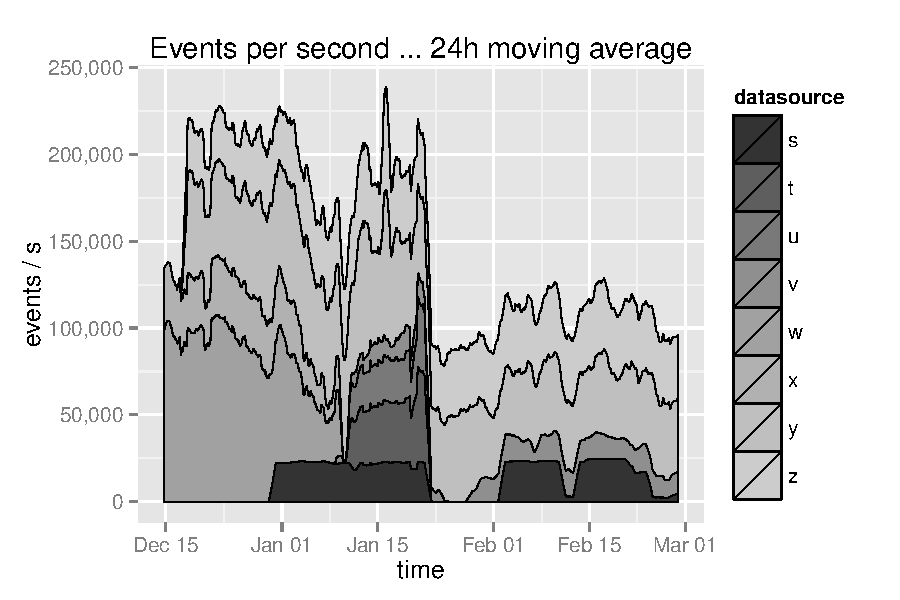
\includegraphics[width = 2.3in]{ingestion_rate}
\caption{Combined cluster ingestion rates.}
\label{fig:ingestion_rate}
\end{figure}

For the given datasources, the number of dimensions vary from 5 to 35, and the
number of metrics vary from 2 to 24. The peak ingestion latency we measured in
production was 22914.43 events/second/core on a datasource with 30 dimensions
and 19 metrics.

The latency measurements we presented are sufficient to address the our stated
problems of interactivity. We would prefer the variability in the latencies to
be less, which can be achieved by adding additional
hardware, but we have not chosen to do so because of cost concerns.

\section{Demonstration Details}

We would like to do an end-to-end demonstratation of Druid, from setting up a
cluster, ingesting data, structuring a query, and obtaining results. We would
also like to showcase how to solve real-world data analysis problems with Druid
and demonstrate tools that can be built on top of it, including interactive
data visualizations, approximate algorithms, and machine-learning components.
We already use similar tools in production.

\subsection{Setup}

Users will be able to set up a local Druid cluster to better understand the
components and architecture of the system. Druid is designed to run on
commodity hardware and Druid nodes are simply java processes that need to be
started up. The local setup will allow users to ingest data from Twitter's
public API and query it.  We will also provide users access to an AWS hosted
Druid cluster that contains several terabytes of Twitter data that we have been
collecting for over 2 years. There are over 3 billion tweets in this data set,
and new events are constantly being ingested. We will walk through a variety of
different queries to demonstrate Druid's arbitrary data-exploration
capabilities.

Finally, we will teach users how to build a simple interactive dashboard on top
of Druid. The dashboard will use some of Druid's more powerful features such as
approximate algorithms for quickly determining the cardinality of sets, and
machine learning algorithms for scientific computing problems such as anomaly
detection.  These use cases represent some of the more interesting problems we
use Druid for in production.

\subsection{Goals}

We will not only walk users through solving real-world problems with Druid and
different tools that have been built on top of Druid, but also answer
conference-specific questions such as what are the trending tweets and topics
at VLDB, what netizens are conversing about in the general area, and even
perform a sentiment analysis of VLDB. Our goal is to clearly explain why the
architecture of Druid makes it highly optimal for certain types of queries, and
the potential of the system as a real-time analytics platform.

%\end{document}  % This is where a 'short' article might terminate

% ensure same length columns on last page (might need two sub-sequent latex runs)
\balance

%ACKNOWLEDGMENTS are optional
\section{Acknowledgments}
Druid could not have been built without the help of many great people in the
community.  We want to thank everyone that has contributed to the Druid
codebase for their invaluable support.

% The following two commands are all you need in the
% initial runs of your .tex file to
% produce the bibliography for the citations in your paper.
\bibliographystyle{abbrv}
\bibliography{druid_demo}  % vldb_sample.bib is the name of the Bibliography in this case
% You must have a proper ".bib" file
%  and remember to run:
% latex bibtex latex latex
% to resolve all references

\end{document}
